Jeg syntes ikke at det er lett å definere de konkrete karriereveiene en fra MTKJ kan ta. Til tross for det skal jeg forsøke å snakke litt om hver av disse veiene, og her kommer sikkert mange til å være uenig med meg, men synd for deg. Noen bransjer sier seg selv, men andre er svært diffuse. Jeg tenker å starte med den mest diffuse karriereveien: konsulent. 

\section{Konsulent}

Etter min mening så finnes det hovedsakelig 3 typer konsulenter når man er utdannet som siving. ved NTNU. Disse ulike konsulentene er i realiteten svært forskjellige, men fellesnevneren er at de utenlukkende jobber for andre bedrifter ved å leie ut de ansatte. Det fører til at konsulenter kan jobbe med svært varierte prosjekter og ha mye å gjøre i gode perioder, men også at man kan ende opp med å sitte på benk i dårlige perioder (du har ingen prosjekt og tar kurs eller jobber med interne prosjekter).

\begin{figure}[H]
    \centering
    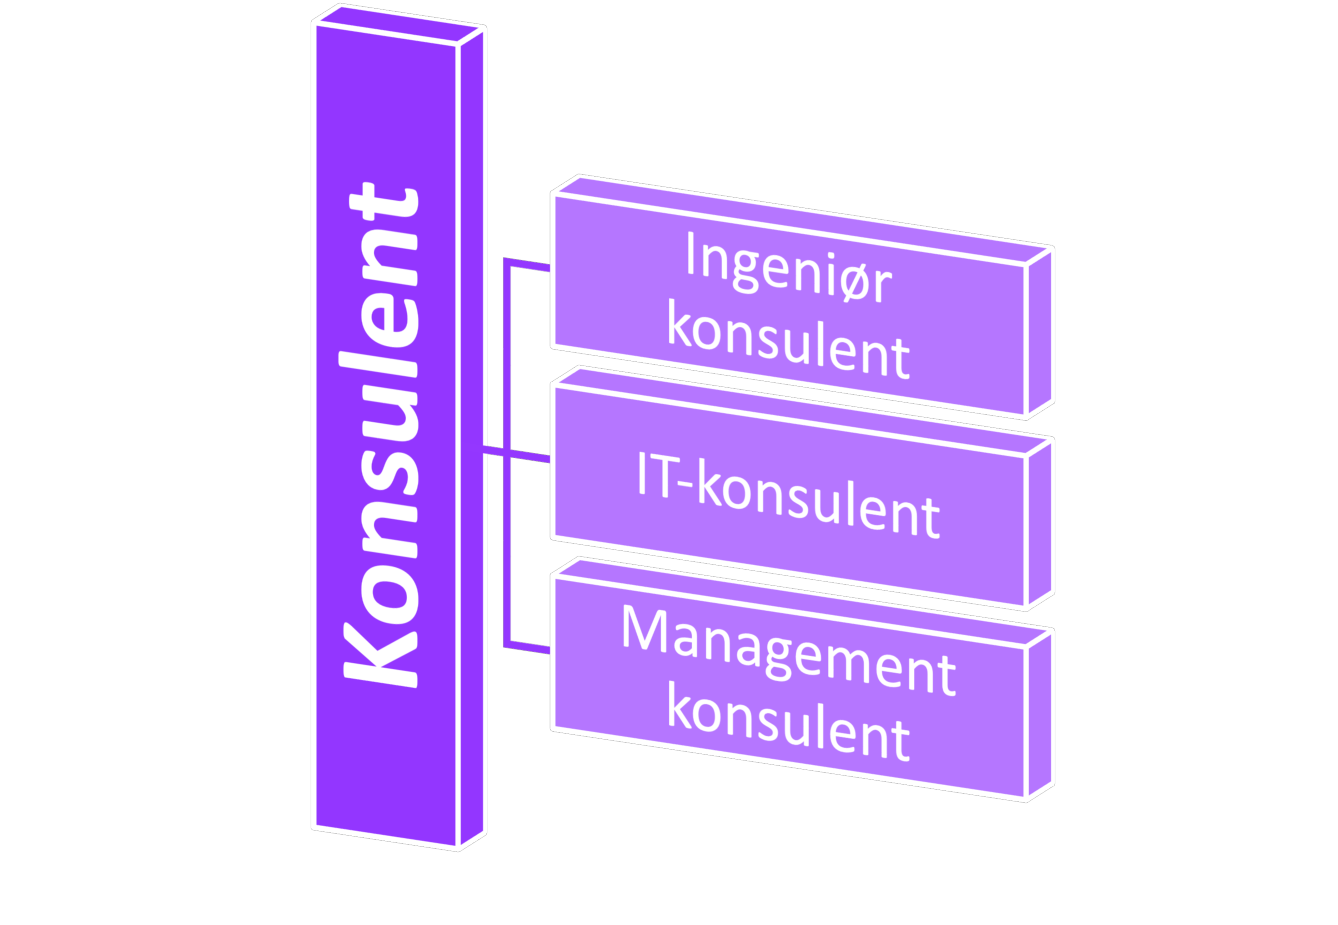
\includegraphics[width=0.5\linewidth]{images/Konsulent.pdf}
\end{figure}



\subsection{Ingeniør konsulent}

Jeg er usikker på hvor jeg har hørt dette begrepet eller om jeg fant på det selv, men en ingeniør konsulent er betegnelsen jeg velger å bruke om folk fra følgende selskaper:

\begin{figure}[H]
    \centering
    \includegraphics[width=1\linewidth]{images/Ingeniør-Konsulent.pdf}
    \caption{Oversikt over såkalte \textit{Ingeniør konsulent} bedrifter, sortert etter antall ansatte.}
    \label{fig:ingeniør-konsulent}
\end{figure}

Selskapene omtales også som bygg og anlegg ettersom disse selskapene hovedsakelig prosjekterer konstruksjoner og leier ut sine konsulenter (også kalt rådgivere). Siden mange selskaper er skandinaviske så refereres de ansatte til som rådgivere, men betydningen er det samme. Typiske oppgaver de driver med er prosjektering av karbonfangstanlegg, bygge vindparker og den type ingeniørarbeid. Denne typen konsulent er derfor mye mer teknisk og samsvarer mer med hva man studerte på Gløs enn de andre typene konsulenter. 



\subsection{IT-konsulent}

Det finnes svært mange IT-konsulentselskaper og de holder hovedsakelig på med å leie ut sine ansatte for IT-prosjekter. Disse prosjektene kan være å bygge opp et system for Equinor eller å bistå Trøndelag med Helseplattformen - Altså alt som har noe med IT å gjøre. Det er høy turnover i både IT-konsulentbransjen og managementkonsulentbransjen, noe som betyr at de ansatte typisk ikke er lenge i bransjen. Dette er fordi man kan hoppe fra prosjekt til prosjekt som IT-konsulent, hvor noen varer i uker, mens andre kan vare i måneder eller år. Det som ofte kan skje, er at man blir lei av å bytte prosjekt så ofte og mange velger derfor å heller bytte jobb til den kunden man jobber for. Grunnet høy turnover så er IT-konsulentselskaper helt rå på rekruttering. Derfor holder de masse bedpres, er veldig på med å finne graduates og kan ofte tilby heltidsjobb etter endt sommerjobb. Eksempelvis kan Sopra Steria ta imot over 200 nyutdannede og kaste dem ut i prosjekter de aldri har hold på med før. IT-konsulentbedriftene er derfor helt rå på opplæring og derfor settes det mer vekt på lærevillighet enn hva du nødvendigvis kan. Tanken er at hvis du er flink på Gløs og klarer å lære alt fra fluidmekanikk til numerisk matematikk, så klarer man å lære seg det som trengs i IT-bransjen relativt lett.

\begin{figure}[H]
    \centering
    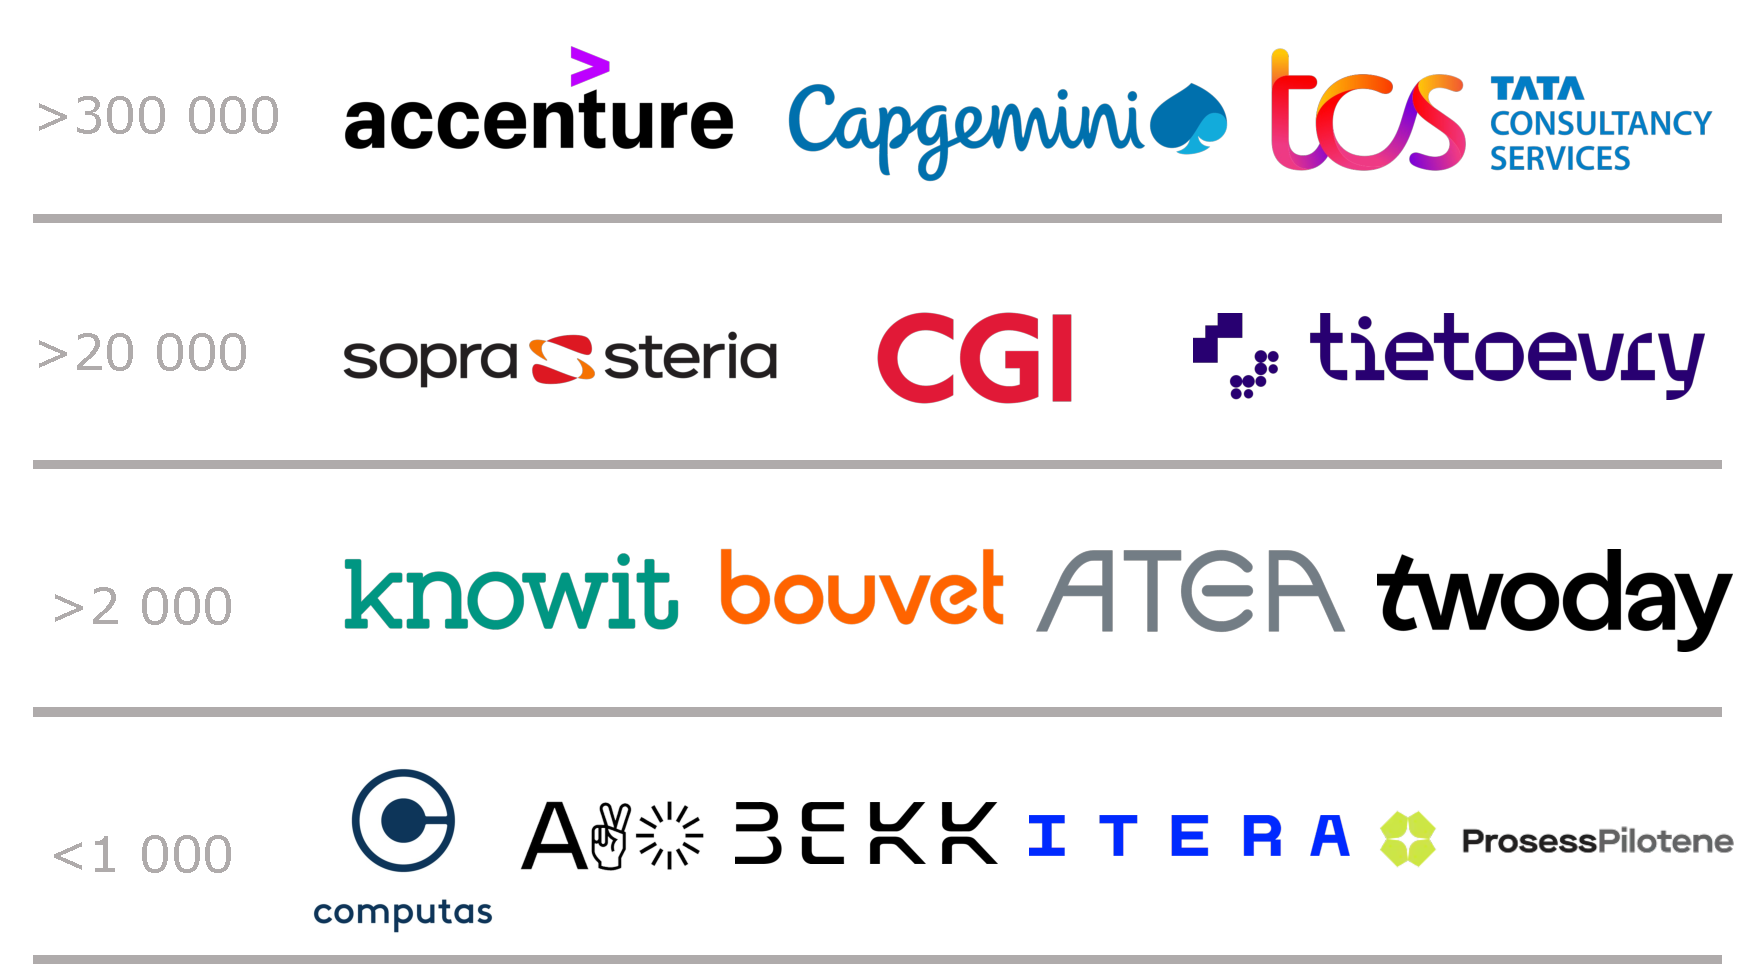
\includegraphics[width=1\linewidth]{images/IT-konsulent.pdf}
    \caption{Oversikt over utvalgte IT-konsulentselskaper, sortert etter antall ansatte.}
    \label{fig:enter-label}
\end{figure}

Listen med IT-konsulentselskaper er ikke komplett ettersom det finnes utallig mange aktører. Jeg har valgt ut noen av de som er mer kjent og av ulike størrelser. Det finnes derfor mange flere IT-konsulentselskaper enn det gjør innen bygg og anlegg. Det som også er verdt å merke seg er at disse selskapene er mye mer internasjonale, noe som fører til at størrelsen til noen av dem er helt enorme (f.eks. Accenture).



\subsection{Management konsulent}

En management konsulent kan kategoriseres som de konsulentene som verken driver med ingeniørarbeid eller direkte IT-tjenester. Det er derfor den vanskeligste rollen å definere fordi det er så mangt. Slike konsulenter ser ofte på hvilken skole du kommer fra og ikke så mye om du går EMIL eller Kyb. Derimot så er de svært ettertraktet siden både ingeniører, økonomer og samfunnsvitere kan bli management konsulenter. Derfor kan typiske arbeidsoppgaver handle om å definere selskapsstrategier eller investeringsbeslutninger osv. Du kan få en oppgave fra Posten om å definere satsningsområder, hjelpe Hafslund gjennom et oppkjøp av et annet selskap eller hjelpe en start-up med å vokse og stå på sine egne bein. 

\begin{figure}[H]
    \centering
    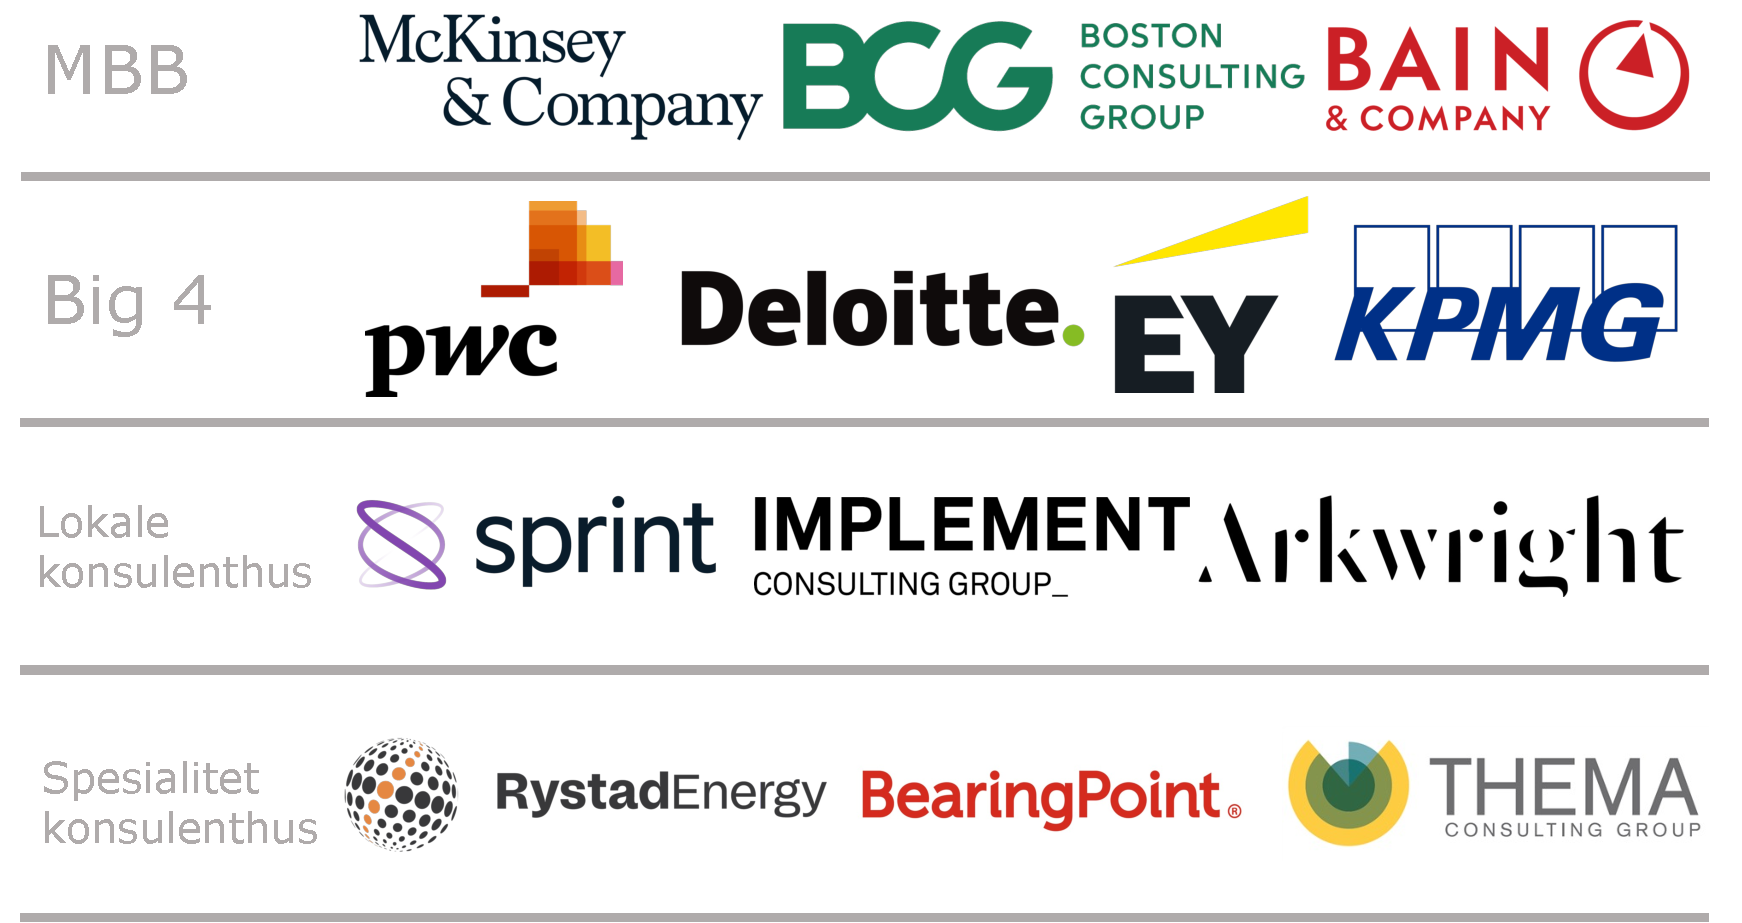
\includegraphics[width=1\linewidth]{images/Manage-Konsulent.pdf}
    \caption{Oversikt over management konsulentselskaper sortert etter kategori.}
    \label{fig:enter-label}
\end{figure}

Siden slike konsulenter kan drive med så mye så deles de ofte inn i ulike kategorier som vist over. \textbf{MBB} står for \textit{McKinsey, BCG og Bain} og er anerkjent som de mest prestisjefulle konsulentselskapene å jobbe hos, også kalt for \textit{Tier 1}. De rekrutterer kun fra toppsjiktet, altså folk med toppkarakterer fra Gløs for eksempel. De er også internasjonalt anerkjent og forbindes med status. McKinsey er den største og de er veldig hemmelighetsfulle om sine kunder, men f.eks. serien \textit{Dopesick} (Disney+) handler om hvordan McKinsey-konsulenter arbeidet med Purdue Pharma for å drive salget av OxyContin, til tross for økende bevis på at medisinen var sterkt avhengighetsskapende og en drivkraft bak opioidkrisen. \textbf{Big 4}, eller de fire store, er gigantiske selskaper som hovedsakelig består av revisorer. De er med i denne oversikten ettersom denne bransjen krever at man er i kontakt med mange selskaper, så derfor driver de også med konsulenttjenester. De var tidligere mye større på konsulentsiden, men en lov fra USA, Sarbanes–Oxley Act, førte til at mange måtte selge sine konsulenttjenester. På den tiden var det faktisk Big 5, men den siste ble tatt i ulovlig shit og forsvant. PwC sine konsulenttjenester ble solgt til IBM, EY til Capgemini og KPMG til Bearingpoint. 

I motsetning til MBB som sender et fåtall konsulenter til et prosjekt, kan Big 4 sende flere titalls. Derfor kan Big 4 ofte jobbe med implementeringsprosjekter som krever mange hoder, mens MBB fokuserer mye mer på den overordnende strategien. \textbf{Lokale konsulenthus} defineres av å være norske eller skandinaviske og driver mye med det MBB holder på med, bare på et lokalt nivå. Den siste kategorien er \textbf{Spesialitet konsulenthus}, altså de som er gode på et konkret område. Eksempelvis er Rystad Energy svært gode innen energianalyse, mens Thema er gode på strømmarkedet i Norden. 

Det er verdt å nevne at siden de fleste av konsulentselskapene er utenlandske så følger de ikke-norske prinsipper. Det er eksempelvis vanlig å bli <<rangert>> eller at de setter karakter på hvor dyktig du har vært. De fleste blir satt i midten, mens de som virkelig fortjener det får topp og de som underpresterer får ofte dårligere karakterer. Dette er for å gi deg tilbakemelding på hvordan du kan bli bedre, men karakteren teller ofte på hvor mye bonus du får. Les mer på E24 \cite{e24_talentfabrikkene}.

\begin{figure}[H]
    \centering
    
\includegraphics[width=0.5\linewidth]{images/konsulent_meme.png}
\end{figure}


\section{Industri}

Det er lett for meg å kategorisere karriereveier som enten konsulent eller industri, men sånn får det bli. Poenget er at disse industribedriftene jobber med ganske konkrete ting, som sier seg selv, mens konsulentene krever mer forklaring. Det finnes et betydelig antall fra MTKJ som jobber i konsulentbransjen, men det er absolutt flest innen industrien. Derfor vil følgende liste med bedrifter være en god representasjon av karriereveier (jeg tør å påstå at 90\% av MTKJ-ere er i disse selskapene).

\begin{figure}[H]
    \centering
    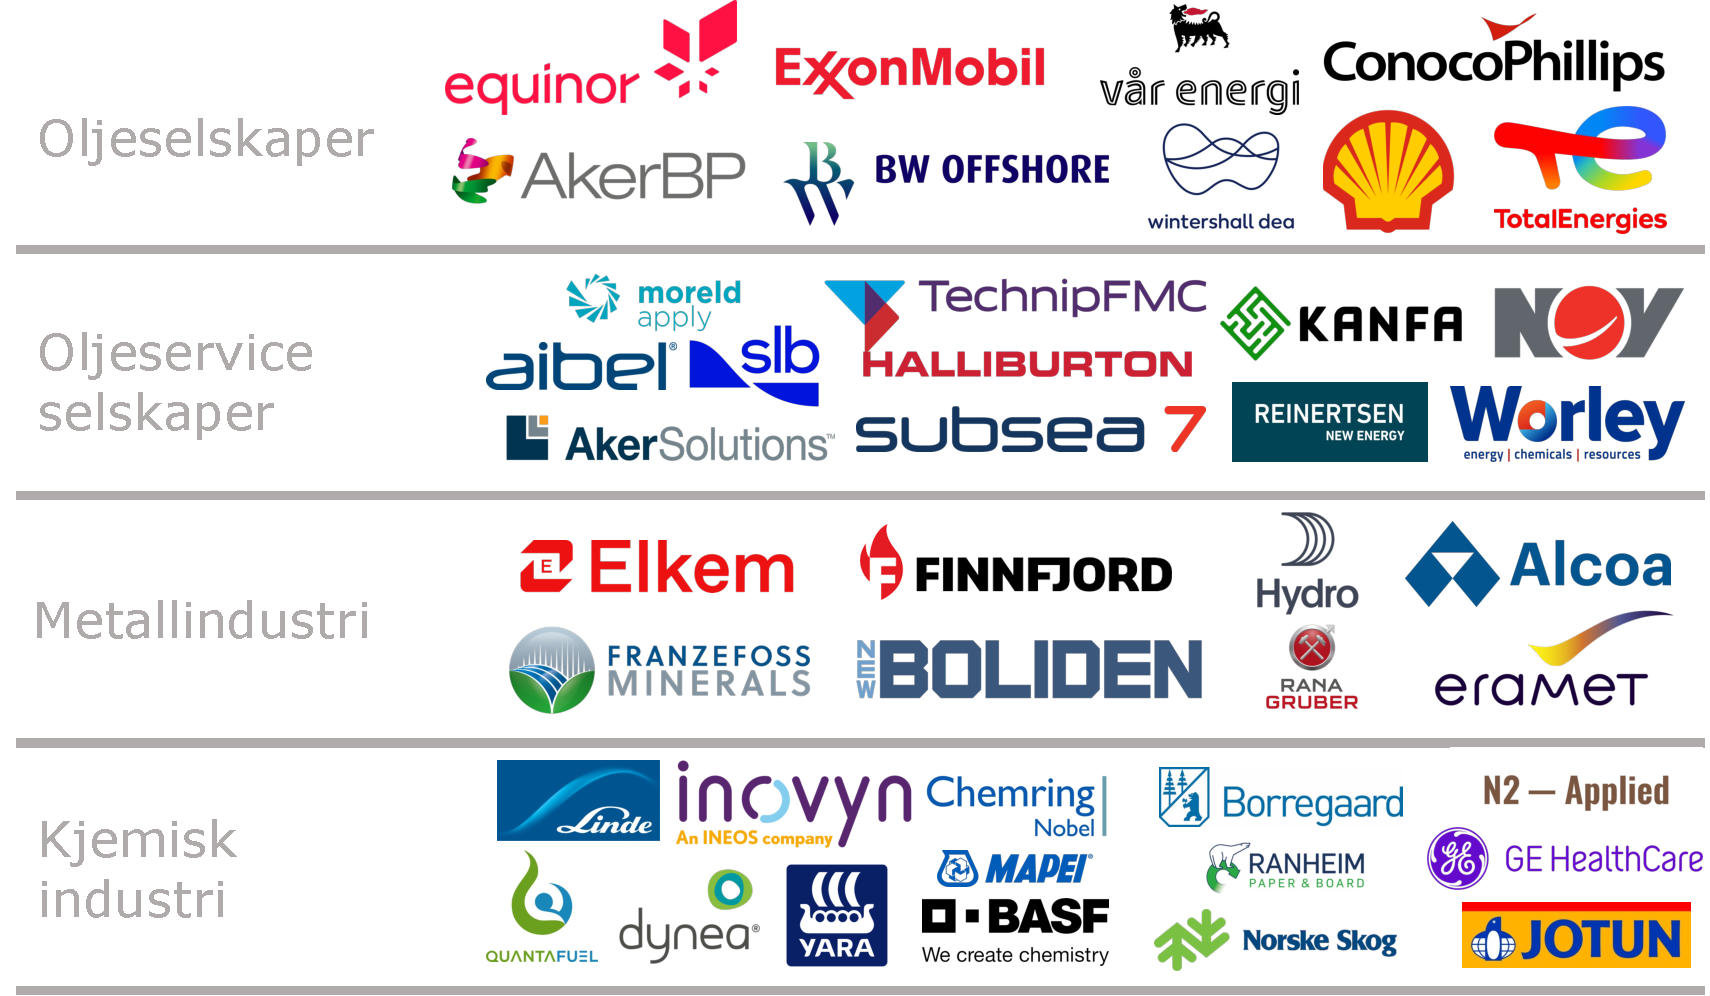
\includegraphics[width=1\linewidth]{images/Industri1.pdf}
    \caption{Industri, del 1}
    \label{fig:industri1}
\end{figure}

\textbf{Oljeselskaper} kjenner nok de fleste til. De driver gjerne med utvinning av olje og gass. \textbf{Oljeservice selskaper} derimot, jobber tett mot oljeselskapene og kan bistå med bygging og ulike tekniske løsninger. For eksempel så er Aker BP operatør, mens Aker Solutions bistår med alt annet rundt. \textbf{Metallindustri} sier også seg selv med at de produserer metaller. Hydro produserer aluminium, Eramet produserer ferromangan osv. I Norge er det veldig mange slike selskaper, men de ligger ofte langt fra store byer. \textbf{Kjemisk industri} produserer derimot kjemiske produkter og her er spennet svært bredt. Det kan være røntgenkontrastmidler fra GE Healthcare til gjødsel fra Yara. 

\begin{figure}[H]
    \centering
    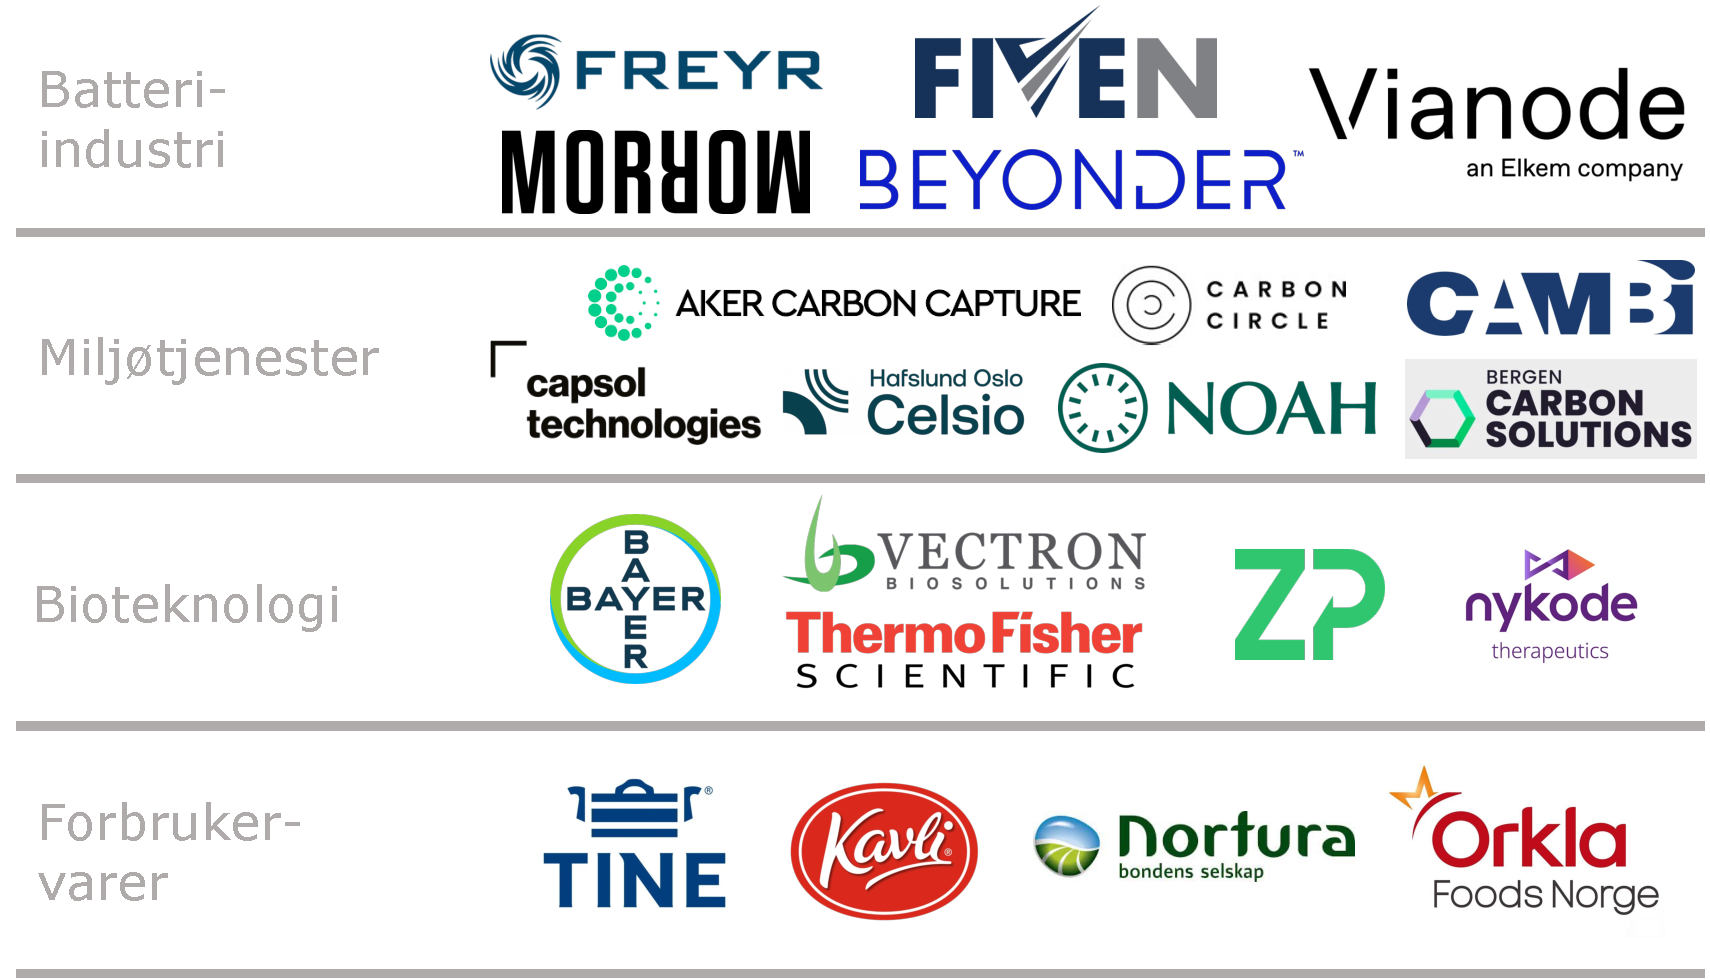
\includegraphics[width=1\linewidth]{images/Industri2.pdf}
    \caption{Industri, del 2}
    \label{fig:industri2}
\end{figure}

Den neste kategorien er \textbf{batteriindustri}, og den sier også seg selv da de produserer batterier, men dette er en relativ ny industri i Norge og derav under konstant utvikling. \textbf{Miljøtjenester} har jeg kalt selskaper som jobber med alt fra karbonfangst til avfallshåndtering. \textbf{Bioteknologi} har jeg kalt de som driver med medisinsk forskning og sånt. \textbf{Forbrukervarer} trenger jeg ikke å forklare.

\begin{figure}[H]
    \centering
    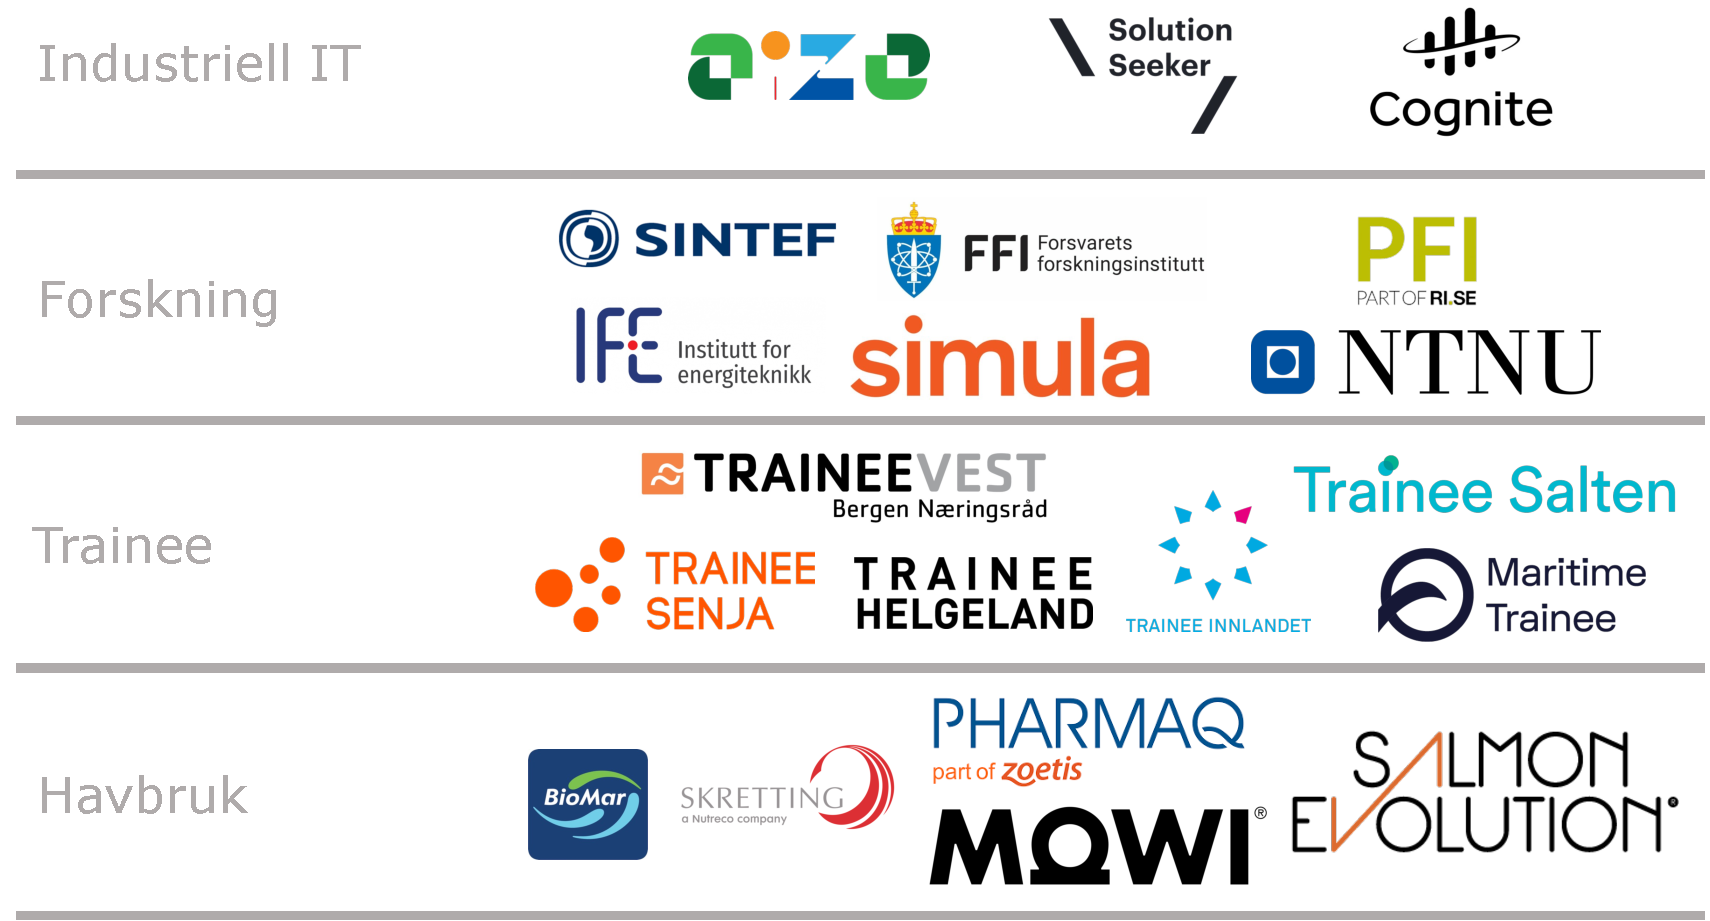
\includegraphics[width=1\linewidth]{images/Industri3.pdf}
    \caption{Industri, del 3}
    \label{fig:industri3}
\end{figure}

\textbf{Industriell IT} har jeg kalt de som utelukkende bistår industrien med IT-løsninger. Cognite eies av Aker og driver med masse fancy maskinlæring til Aker BP.
\textbf{Forskning} er kanskje feil å kategorisere som en industri, men det får gå. Her er det verdt å merke at det er en vesentlig forskjell mellom NTNU og f.eks. SINTEF ettersom SINTEF er et privat selskap, mens NTNU er offentlig. Derfor er det store forskjeller innad i denne kategorien. \textbf{Trainee} er en kategori som består av ulike traineepropgram overalt i Norge. Mange selskaper har opplegg hvor man roterer mellom avdelinger, mens disse traineeprogrammene er mellom ulike selskaper. De finnes ofte for å tiltrekke seg unge til mindre ettertraktede steder. \textbf{Havbruk} jobber med fisk og den verdikjeden der da, ellernoe sånt. 

\begin{figure}[H]
    \centering
    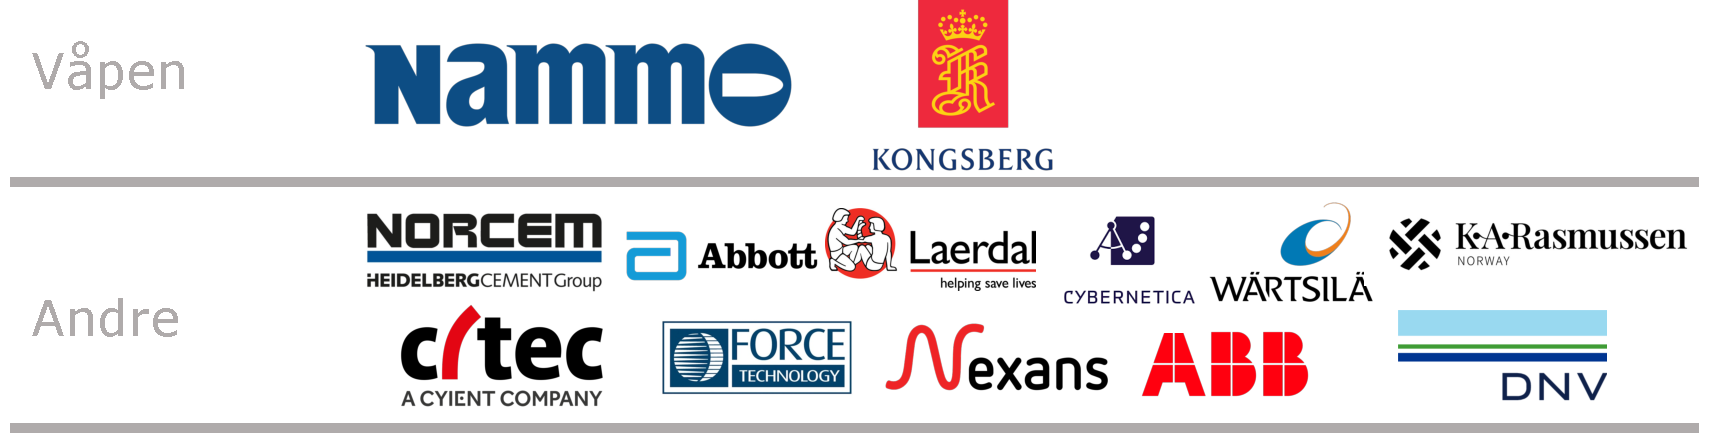
\includegraphics[width=1\linewidth]{images/Industri4.pdf}
    \caption{Industri, del 4}
    \label{fig:industri4}
\end{figure}

\textbf{Våpen} lager jo, våpen. Og den siste kategorien \textbf{Andre} er de jeg ikke klarer å få til å passe inn i eksisterende kategorier. Norcem lager sement, men det er jo ikke direkte kjemisk industri? DNV driver med standarder og regelverk, passer jo heller ikke inn i de andre. 